\documentclass{standalone}
\usepackage{tikz}
\usetikzlibrary{patterns, positioning}

\begin{document}
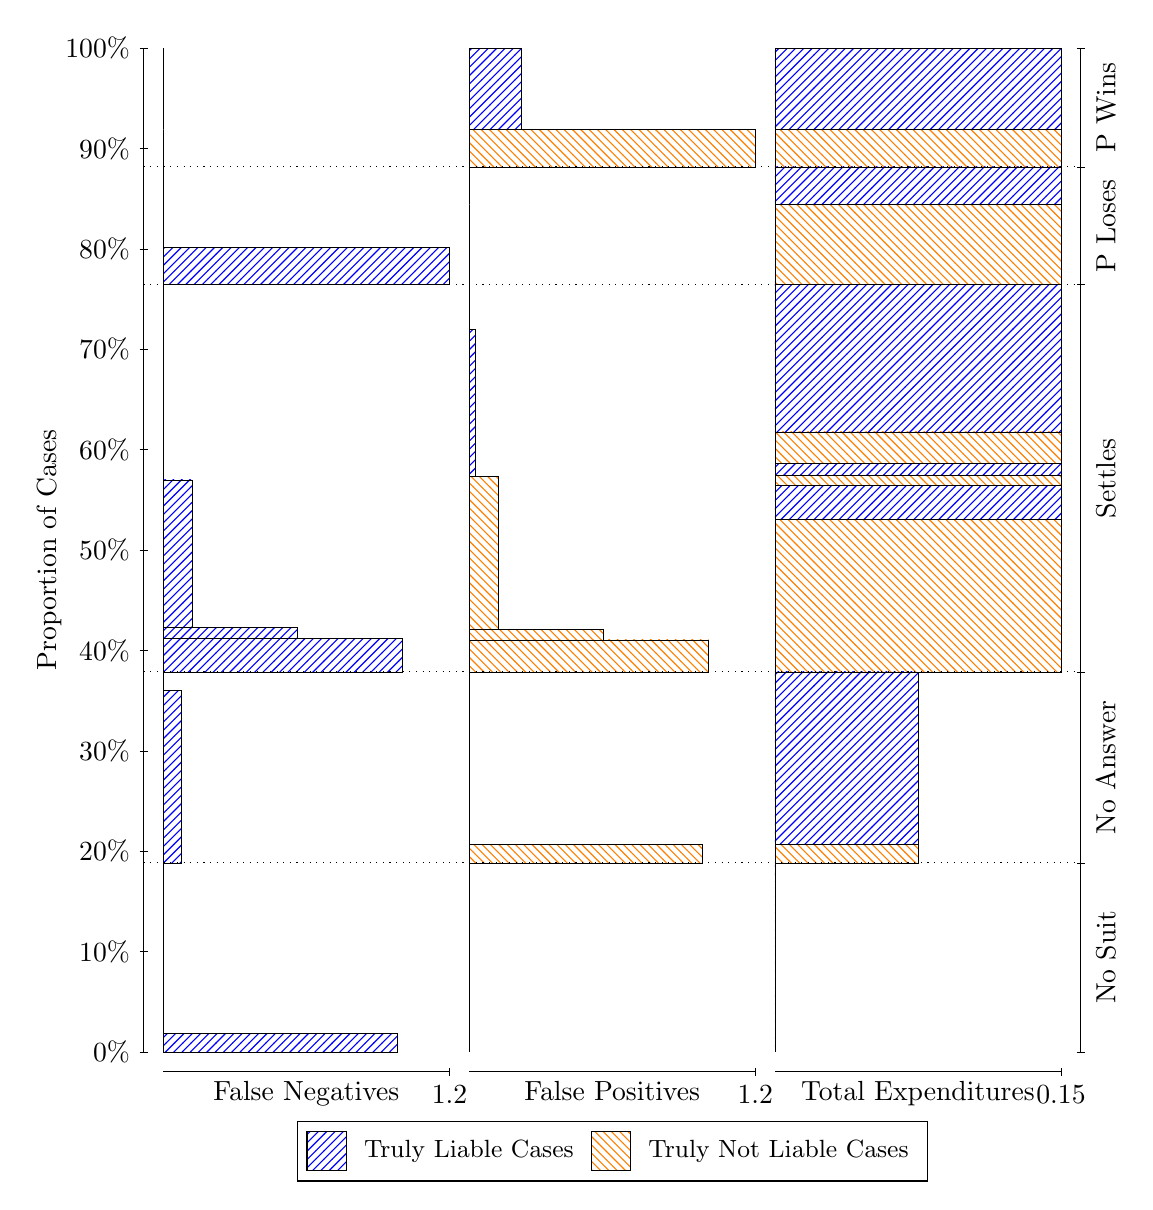
\begin{tikzpicture}
\draw[black, very thin] (1.5,1.75) -- (1.5,14.5);
\node[rotate=90, anchor=center] at (0.3, 8.125) {Proportion of Cases};
\draw[black, very thin] (1.45,1.75) -- (1.55,1.75);
\node[anchor=east] at (1.45, 1.75) {0\%};
\draw[black, very thin] (1.45,3.025) -- (1.55,3.025);
\node[anchor=east] at (1.45, 3.025) {10\%};
\draw[black, very thin] (1.45,4.3) -- (1.55,4.3);
\node[anchor=east] at (1.45, 4.3) {20\%};
\draw[black, very thin] (1.45,5.575) -- (1.55,5.575);
\node[anchor=east] at (1.45, 5.575) {30\%};
\draw[black, very thin] (1.45,6.85) -- (1.55,6.85);
\node[anchor=east] at (1.45, 6.85) {40\%};
\draw[black, very thin] (1.45,8.125) -- (1.55,8.125);
\node[anchor=east] at (1.45, 8.125) {50\%};
\draw[black, very thin] (1.45,9.4) -- (1.55,9.4);
\node[anchor=east] at (1.45, 9.4) {60\%};
\draw[black, very thin] (1.45,10.675) -- (1.55,10.675);
\node[anchor=east] at (1.45, 10.675) {70\%};
\draw[black, very thin] (1.45,11.95) -- (1.55,11.95);
\node[anchor=east] at (1.45, 11.95) {80\%};
\draw[black, very thin] (1.45,13.225) -- (1.55,13.225);
\node[anchor=east] at (1.45, 13.225) {90\%};
\draw[black, very thin] (1.45,14.5) -- (1.55,14.5);
\node[anchor=east] at (1.45, 14.5) {100\%};

\draw[black, very thin] (13.4,1.75) -- (13.4,14.5);
\draw[black, very thin] (13.35,1.75) -- (13.45,1.75);
\node[anchor=west] at (13.35, 1.75) {};
\draw[black, very thin] (13.35,4.1507) -- (13.45,4.1507);
\node[anchor=west] at (13.35, 4.1507) {};
\draw[black, very thin] (13.35,6.5779) -- (13.45,6.5779);
\node[anchor=west] at (13.35, 6.5779) {};
\draw[black, very thin] (13.35,11.494) -- (13.45,11.494);
\node[anchor=west] at (13.35, 11.494) {};
\draw[black, very thin] (13.35,12.99) -- (13.45,12.99);
\node[anchor=west] at (13.35, 12.99) {};
\draw[black, very thin] (13.35,14.5) -- (13.45,14.5);
\node[anchor=west] at (13.35, 14.5) {};

\draw[black, very thin, pattern color=blue, pattern=north east lines] (1.75,1.75) rectangle (4.716,1.991);
\draw[black, very thin, pattern color=orange, pattern=north west lines] (1.75,1.991) rectangle (1.75,4.1507);
\draw[black, very thin, pattern color=blue, pattern=north east lines] (1.75,4.1507) rectangle (1.9724,6.338);
\draw[black, very thin, pattern color=orange, pattern=north west lines] (1.75,6.338) rectangle (1.75,6.5779);
\draw[black, very thin, pattern color=blue, pattern=north east lines] (1.75,6.5779) rectangle (4.7901,7.0038);
\draw[black, very thin, pattern color=blue, pattern=north east lines] (1.75,7.0038) rectangle (3.4554,7.1448);
\draw[black, very thin, pattern color=blue, pattern=north east lines] (1.75,7.1448) rectangle (2.1207,9.0141);
\draw[black, very thin, pattern color=orange, pattern=north west lines] (1.75,9.0141) rectangle (1.75,11.494);
\draw[black, very thin, pattern color=blue, pattern=north east lines] (1.75,11.494) rectangle (5.3833,11.968);
\draw[black, very thin, pattern color=orange, pattern=north west lines] (1.75,11.968) rectangle (1.75,12.99);
\draw[black, very thin, pattern color=orange, pattern=north west lines] (1.75,12.99) rectangle (1.75,13.463);
\draw[black, very thin, pattern color=blue, pattern=north east lines] (1.75,13.463) rectangle (1.75,14.5);
\draw[black, very thin, pattern color=orange, pattern=north west lines] (5.6333,1.75) rectangle (5.6333,3.9097);
\draw[black, very thin, pattern color=blue, pattern=north east lines] (5.6333,3.9097) rectangle (5.6333,4.1507);
\draw[black, very thin, pattern color=orange, pattern=north west lines] (5.6333,4.1507) rectangle (8.5993,4.3906);
\draw[black, very thin, pattern color=blue, pattern=north east lines] (5.6333,4.3906) rectangle (5.6333,6.5779);
\draw[black, very thin, pattern color=orange, pattern=north west lines] (5.6333,6.5779) rectangle (8.6735,6.9823);
\draw[black, very thin, pattern color=orange, pattern=north west lines] (5.6333,6.9823) rectangle (7.3388,7.1209);
\draw[black, very thin, pattern color=orange, pattern=north west lines] (5.6333,7.1209) rectangle (6.0041,9.0578);
\draw[black, very thin, pattern color=blue, pattern=north east lines] (5.6333,9.0578) rectangle (5.7075,10.927);
\draw[black, very thin, pattern color=blue, pattern=north east lines] (5.6333,10.927) rectangle (5.6333,11.494);
\draw[black, very thin, pattern color=orange, pattern=north west lines] (5.6333,11.494) rectangle (5.6333,12.516);
\draw[black, very thin, pattern color=blue, pattern=north east lines] (5.6333,12.516) rectangle (5.6333,12.99);
\draw[black, very thin, pattern color=orange, pattern=north west lines] (5.6333,12.99) rectangle (9.2667,13.463);
\draw[black, very thin, pattern color=blue, pattern=north east lines] (5.6333,13.463) rectangle (6.3007,14.5);
\draw[black, very thin, pattern color=orange, pattern=north west lines] (9.5167,1.75) rectangle (9.5167,3.9097);
\draw[black, very thin, pattern color=blue, pattern=north east lines] (9.5167,3.9097) rectangle (9.5167,4.1507);
\draw[black, very thin, pattern color=orange, pattern=north west lines] (9.5167,4.1507) rectangle (11.333,4.3906);
\draw[black, very thin, pattern color=blue, pattern=north east lines] (9.5167,4.3906) rectangle (11.333,6.5779);
\draw[black, very thin, pattern color=orange, pattern=north west lines] (9.5167,6.5779) rectangle (13.15,8.5148);
\draw[black, very thin, pattern color=blue, pattern=north east lines] (9.5167,8.5148) rectangle (13.15,8.9407);
\draw[black, very thin, pattern color=orange, pattern=north west lines] (9.5167,8.9407) rectangle (13.15,9.0793);
\draw[black, very thin, pattern color=blue, pattern=north east lines] (9.5167,9.0793) rectangle (13.15,9.2203);
\draw[black, very thin, pattern color=orange, pattern=north west lines] (9.5167,9.2203) rectangle (13.15,9.6247);
\draw[black, very thin, pattern color=blue, pattern=north east lines] (9.5167,9.6247) rectangle (13.15,11.494);
\draw[black, very thin, pattern color=orange, pattern=north west lines] (9.5167,11.494) rectangle (13.15,12.516);
\draw[black, very thin, pattern color=blue, pattern=north east lines] (9.5167,12.516) rectangle (13.15,12.99);
\draw[black, very thin, pattern color=orange, pattern=north west lines] (9.5167,12.99) rectangle (13.15,13.463);
\draw[black, very thin, pattern color=blue, pattern=north east lines] (9.5167,13.463) rectangle (13.15,14.5);
\draw[black, dotted] (1.5,4.1507) -- (13.4,4.1507);
\draw[black, dotted] (1.5,6.5779) -- (13.4,6.5779);
\draw[black, dotted] (1.5,11.494) -- (13.4,11.494);
\draw[black, dotted] (1.5,12.99) -- (13.4,12.99);
\draw[black, very thin] (1.75,1.5) -- (5.3833,1.5);
\node[anchor=north] at (3.5667, 1.5) {False Negatives};
\draw[black, very thin] (5.3833,1.45) -- (5.3833,1.55);
\node[anchor=north] at (5.3833, 1.45) {1.2};

\draw[black, very thin] (5.6333,1.5) -- (9.2667,1.5);
\node[anchor=north] at (7.45, 1.5) {False Positives};
\draw[black, very thin] (9.2667,1.45) -- (9.2667,1.55);
\node[anchor=north] at (9.2667, 1.45) {1.2};

\draw[black, very thin] (9.5167,1.5) -- (13.15,1.5);
\node[anchor=north] at (11.333, 1.5) {Total Expenditures};
\draw[black, very thin] (13.15,1.45) -- (13.15,1.55);
\node[anchor=north] at (13.15, 1.45) {0.15};

\node[black, centered, rotate=90] at (13.72, 2.9503) {No Suit};
\node[black, centered, rotate=90] at (13.72, 5.3643) {No Answer};
\node[black, centered, rotate=90] at (13.72, 9.036) {Settles};
\node[black, centered, rotate=90] at (13.72, 12.242) {P Loses};
\node[black, centered, rotate=90] at (13.72, 13.745) {P Wins};

\draw (7.449999999999999,1.5) node[draw=none] (baseCoordinate) {};
\begin{scope}[align=center]
        \matrix[scale=0.5, draw=black, below=0.5cm of baseCoordinate, nodes={draw}, column sep=0.1cm]{
            \node[rectangle, draw, minimum width=0.5cm, minimum height=0.5cm, pattern=north east lines, pattern color=blue] {}; &
            \node[draw=none, font=\small] (B) {Truly Liable Cases}; &
            \node[rectangle, draw, minimum width=0.5cm, minimum height=0.5cm, pattern=north west lines, pattern color=orange] {}; &
            \node[draw=none, font=\small] (B) {Truly Not Liable Cases}; \\
            };
\end{scope}

\end{tikzpicture}
\end{document}